\section{ギャップを仮定しない推定バイアスの鋭い境界}\label{sec:gapfree}
固有空間への幾何収束と、フィルタ後の平均から最小値を推定することは異なる。
目標に近い固有値の確率が残っても、平均のバイアスは小さくなり得る。
以下ではギャップ下界を仮定せず、$0<a<1$、$t\geq1$、最小固有空間への
初期質量をちょうど$a$とする。質量の下界だけが既知の場合も、その下界を
代入した式は上界として有効である。

\begin{theorem}[正確な二点バイアス包絡]\label{thm:envelope}
$\lambda_0<1$、$q$は$[\lambda_0,1]$上の連続で厳密に正の応答とし、
$R_t(x)=[q(x)/q(\lambda_0)]^{2t}$と置く。
最小値が$\lambda_0$で、その初期質量が$a$であるすべての有限スペクトルに
わたる、フィルタ後平均の最大バイアスは
\begin{equation}\label{eq:envelope}
 \mathcal B_t(q;a,\lambda_0)
 =\max_{\lambda_0\leq x\leq1}
 \frac{(1-a)(x-\lambda_0)R_t(x)}{a+(1-a)R_t(x)}
\end{equation}
であり、重み$a,1-a$の二固有値スペクトルで達成される。
これは固定した応答に対する正確な最悪値であり、全フィルタにわたる最適化や
量子queryの下界ではない。
\end{theorem}
\begin{proof}
目標外の重みを$(1-a)\nu_i$、$\sum_i\nu_i=1$と書く。
右辺を$b$とすると、定義から各$x$について
$(1-a)(x-\lambda_0)R_t(x)\leq b[a+(1-a)R_t(x)]$。
これを$\nu_i$で平均し、正の分母で割れば上界を得る。
逆に目標外の全質量を最大点$x$へ置けば等号となる。
$x>\lambda_0$のどこかで値が正になるため、目標質量は正確に$a$とできる。
この帰着は線形分数最適化\cite{CharnesCooper}の初等的な特殊例であり、
新しい最適化原理とは主張しない。
\end{proof}

$q_{\rm G}(x)=\cos(\beta x)$、$q_{\rm D}(x)=\cos(\beta\sqrt{x})$、
$0<\beta<\pi/2$とする。後者はエルミート拡張上の偶cosine変換の右空間応答である。
$k=1,2$について
\begin{equation}\label{eq:constant}
 A_a=\frac{a}{1-a},\quad
 C_k(a)=\max_{y\geq0}\frac{y^{1/k}}{1+A_a e^y},\quad
 y_k=\frac1k+W_0\!\left(\frac{e^{-1/k}}{kA_a}\right)
\end{equation}
と定義する。$W_0$はLambert関数の非負実数分枝であり、最大値は$y=y_k$で得られる。

\begin{theorem}[一様収束率と鋭い漸近定数]\label{thm:rates}
$0\leq\lambda_0<1$と上記の全有限スペクトル・重みについて一様に
\begin{equation}\label{eq:rates}
 \mu_t-\lambda_0\leq
 \begin{cases}
 C_2(a)/(\beta\sqrt{t}), &q=q_{\rm G},\\
 C_1(a)/(\beta^2t), &q=q_{\rm D}
 \end{cases}
\end{equation}
が成立する。固定した$a,\beta$に対し、$\lambda_0=0$、
$x_t=(y_k/(t\beta^2))^{1/k}$の二点スペクトルで、それぞれ$k=2,1$を選ぶと、
上界との比は1へ収束する。
したがって推定器$\alpha\sqrt{\mu_t}$の最悪無雑音誤差の率は、
それぞれ$t^{-1/4}$と$t^{-1/2}$である。
これはスカラー反復回数での比較であり、同一oracle費用での比較ではない。
\end{theorem}
\begin{proof}
$h=-\log q$とする。Gram応答では$h'(x)=\beta\tan(\beta x)\geq\beta^2x$
なので、$d=x-\lambda_0$と書けば
$2t[h(x)-h(\lambda_0)]\geq t\beta^2(x^2-\lambda_0^2)\geq t\beta^2d^2$。
拡張応答では零での連続延長も含め
$h'(x)=\beta\tan(\beta\sqrt{x})/(2\sqrt{x})\geq\beta^2/2$
なので、同じ量は$t\beta^2d$以上となる。
式\eqref{eq:envelope}の分数は$R_t$に関して増加するため、
$R_t\leq e^{-t\beta^2d^k}$を代入し、$y=t\beta^2d^k$と置けば上界を得る。
$C_k$の定義を微分すると$(ky-1)e^y=1/A_a$となり、唯一の解は
式\eqref{eq:constant}である。
一致する下界は$\lambda_0=0$、$x=x_t$を選び、
$2t\log\cos(\beta x_t^{k/2})=-y_k+O(t^{-1})$から得る。
最後に$|\sqrt{\mu_t}-\sqrt{\lambda_0}|\leq\sqrt{\mu_t-\lambda_0}$を用い、
$\lambda_0=0$では等号となる。
\end{proof}

\paragraph{解釈と限界}
最悪スペクトルは$t$ごとに変わる。固定されたギャップのある行列の長時間挙動と
混同しない。固定した正の最小値では両応答とも$h'(\lambda_0)>0$なので、
同じ議論から$\mathcal B_t\leq C_1(a)/(2t h'(\lambda_0))$も得られる。
一方、各有限$t$で目標外固有値を$\lambda_0$へ近づければ、目標忠実度を$a$より
一様に改善することはできない。平均バイアスと状態忠実度の区別が本質的である。
零最小値の例は推定器のバイアス境界の鋭さを示すもので、最小値が既に零と
分かっている問題の困難さを示すものではない。十分速く零へ近づく厳密に正の
最小値でも、連続性により同じ漸近定数が得られる。

受理確率は依然として
$a q(\lambda_0)^{2t}\leq Z_t\leq q(\lambda_0)^{2t}$である。
核があれば$Z_t\geq a$だが、固定した正の最小値では指数的に減少し得る。
よってギャップなしのバイアス保証だけで、一様に効率的な状態準備・推定法は得られない。

\section{正規化、多項式baseline、実装誤差}\label{sec:normalization}
\paragraph{正規化による再試行ペナルティ}
前述のTaylor近似は$P_{m_0}(0)=1$だが、
$\widetilde P_{m_0}(0)=(1+\delta_{m_0})^{-1}$である。
スカラー倍は条件付き分布を変えず、受理確率だけを
$(1+\delta_{m_0})^{-2t}$倍にする。
$\beta=1.2,m_0=1$なら$\delta_{m_0}=0.0864$で、$t=128$での係数は
$6.12\times10^{-10}$となる。固定した正の余裕を毎回掛けると、核がある場合も
理想応答の一定受理確率を失う。これを避けるには
$t\log(1+\delta_{m_0})=O(1)$が必要である。
目標点での正規化を保つ原理自体は既存の多項式projector\cite{LinTongFilter}に
含まれており、ここでは現Taylor近似への具体的な帰結を明示している。

\paragraph{固定次数の参照応答}
$0<\beta<\sqrt2$、$c=\beta^2/2<1$として
\[
 Q_{\rm G}(x)=1-cx^2,\qquad Q_{\rm D}(x)=1-cx
\]
を考える。正規化特異値$s$では$1-cs^4$、$1-cs^2$であり、いずれも偶多項式で
$s\in[-1,1]$上$0$から$1$の範囲にあり、応答レベルでは核を厳密に保存する。
これらは初等的な比較baselineであり、新しい量子アルゴリズムとは主張しない。
$-\log(1-cx^k)$の導関数は$ckx^{k-1}$以上で、局所展開も一致するため、
定理\ref{thm:rates}の上界と鋭い定数がそれぞれ$k=2,1$で同様に成立する。
このスカラー率を得るために理想cosine応答は必須ではない。
次数最適性は示しておらず、実際のQSVT success blockが追加の定数減衰を
導入すれば、再試行ペナルティが再び生じる。

\paragraph{近似success blockへの移行}
縮小作用素$C,\widetilde C$について$\|\widetilde C-C\|\leq E$とし、
$u=C^t\psi$、$Z_t=\|u\|^2>0$とする。望遠和から
$\|\widetilde C^t\psi-u\|\leq tE$、
$|\sqrt{\widetilde Z_t}-\sqrt{Z_t}|\leq tE$を得る。
$tE<\sqrt{Z_t}$なら実装後の受理状態が存在し、規格化後のベクトル距離は
$2tE/\sqrt{Z_t}$以下である。純粋状態のtrace distanceはこの距離以下であり、
$0\leq G\leq I$の期待値差もtrace distance以下なので、Bernoulli読出し誤差が
$\zeta$以下という事象上
\begin{equation}\label{eq:robust}
 |\widehat\sigma-\sigma_0|
 \leq\alpha\sqrt{\mathcal B_t(q;a,\lambda_0)+2tE/\sqrt{Z_t}+\zeta}
\end{equation}
となる。これは条件付き摂動評価であり、新しい安定性原理ではない。
encoding、位相合成、正規化を含む全誤差を$E$へ算入する必要がある。
核では$\sqrt{Z_t}\geq\sqrt a$が利用できるが、正の最小値では許容誤差も
指数的に厳しくなり得る。

\section{鋭い境界の数値監査}\label{sec:envelope-audit}
新規スクリプト\texttt{experiments/qmsve\_gapfree\_envelope.py}は、
一変数の最大化を停留点方程式で解き、seed 20261027の十三準位ランダムスペクトル
計1,000例、および20,001点の格子と独立に照合する。
Lambert式も別のスカラー方程式で照合した。
検査例での上界超過は$2\times10^{-12}$以下だった。
有限検査は実装の確認であり、証明の代替ではない。
JSONに版、基準commit、ソースhash、パラメータ、最大点、受理確率を保存した。

\begin{figure}[tb]
\centering
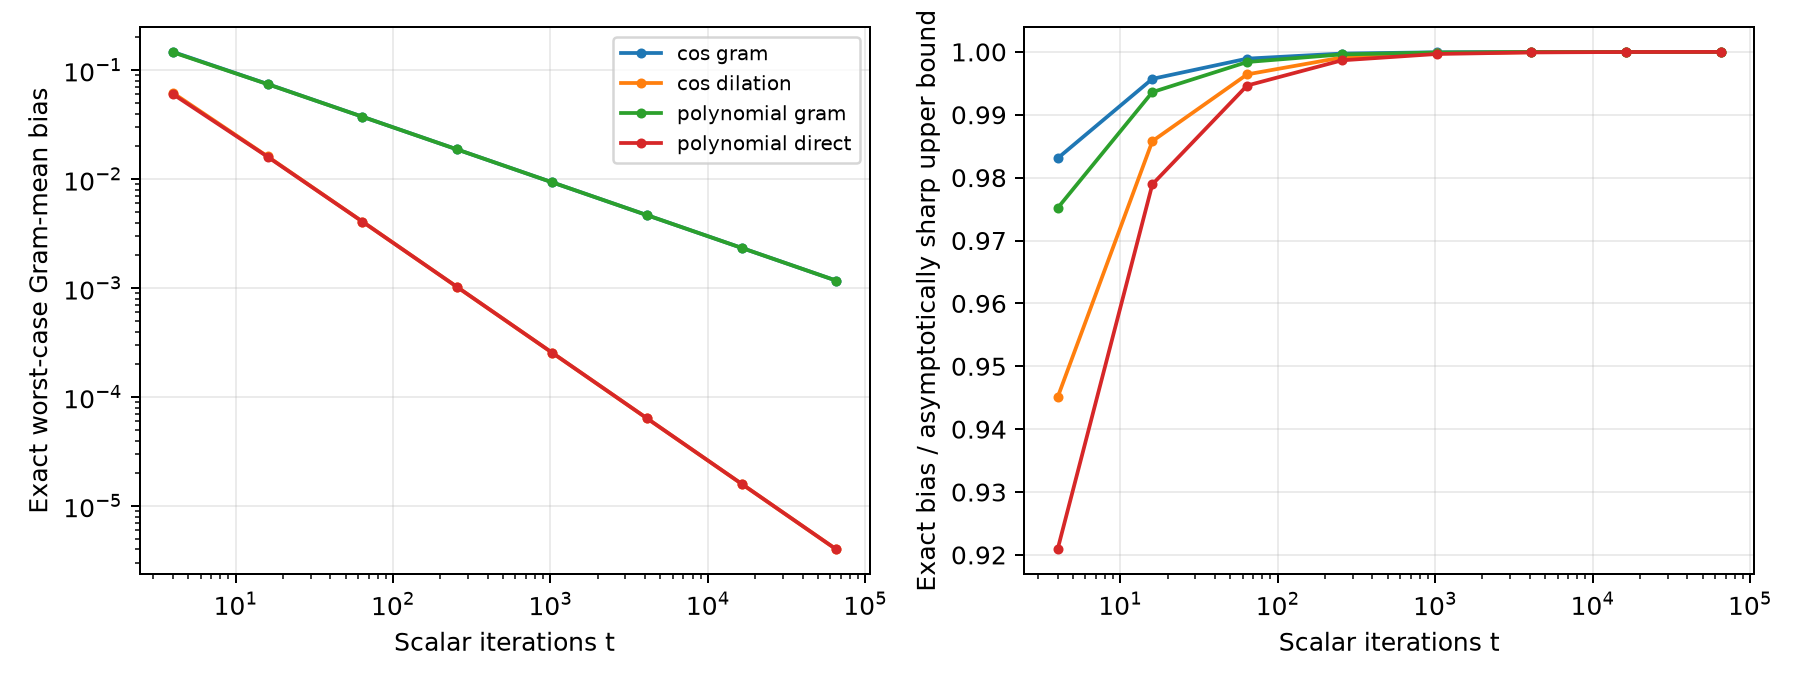
\includegraphics[width=\linewidth]{../../figures/qmsve_gapfree_envelope.png}
\caption{$a=0.4,\beta=1.2$での正確な最悪平均バイアスと、鋭い漸近上界に対する比。
各点は別々の二準位最悪スペクトルを用い、同一行列の軌道ではない。
スカラー反復回数での比較でありoracle費用は揃えていない。}
\end{figure}
$a=0.4$では$C_2(a)=0.360257$、$C_1(a)=0.378089$。
$a=0.1,0.4,0.9$の全四応答は$t=65536$で対応する漸近境界の99.9\%以上に達した。
$a=0.4,t=128$の多項式Gram最悪例では、核保存応答の受理確率は$0.6625$だが、
同一事後分布を持つ全体スケーリング後のTaylor応答では$4.05\times10^{-10}$となる。
これはスケーリングだけの影響を切り分けた比較であり、全回路の比較ではない。
